\documentclass[11pt]{article}
\usepackage[margin=1in]{geometry}
\usepackage{graphicx,booktabs,amsmath,amssymb,hyperref}
\hypersetup{colorlinks=true,urlcolor=blue,citecolor=blue,linkcolor=blue}
\setlength{\parskip}{0.35em}
\setlength{\parindent}{0pt}
\setlength{\emergencystretch}{2em}
\title{Auditing Early-Output Availability and Stopping Costs\\in Frozen Next-Concept Models}
\author{Anytime NCM project\\{\small Internal draft: human authorship and affiliations are not finalized}}
\date{24 October 2026}
\begin{document}
\maketitle
\begin{abstract}
Coarse-to-fine generation offers candidate stopping points, but useful adaptive execution requires acceptable early answers, causal recognition and enough saved work to cover monitoring. We audit these distinctions for released frozen Next-Concept Modeling checkpoints. Historical Sudoku audits find no early exact valid solutions; selected online Sudoku and translation policies reach full depth and add overhead. A new prospective saved-data study searches mixed exit assignments over 128 exploration and 64 reused development WMT14 trajectories. At a fixed budget of 60,000 complete assignment evaluations, a reference-informed development assignment exits early on 18/64 inputs while losing 0.370 BLEU and 0.985 chrF points, within the point tolerances. An uncalibrated monitored-cost surrogate estimates 9.02\% savings, but conditional quality lower bounds fail noninferiority and arbitrary-exit wall latency remains unidentified. A separate saved diagnosis finds early visible text identical to final output on 13/64 development inputs. Thus some early translations exist, while practical adaptive speedup remains unestablished. The finite search is not a certified optimum or a causal policy, and reused development data are not fresh confirmation. We report an inconclusive practical-headroom result and defer unsupported controller/model branches.
\end{abstract}

\section{Question and contribution boundary}
Next-Concept Modeling (NCM) predicts discrete codes in parallel within successive hierarchy levels and reconstructs text from their cumulative representation~\cite{ncm}. We ask whether a frozen released checkpoint can stop different inputs at different levels and improve quality versus actual ready-output latency.

We separate three requirements: \emph{availability} of acceptable early outputs; \emph{recognizability} using only information available at the stopping decision; and \emph{economics}, including reconstruction, decoding, transfers and controller work. Our contribution is a bounded audit separating these requirements, with explicit search, access and uncertainty limits. We introduce no new causal stopping algorithm and claim neither novelty priority nor universal failure of adaptive generation.

The empirical snapshot is repository commit \texttt{39e4533}; historical execution sources and inputs are fixed by their own receipts. The manuscript and source package identify unresolved author metadata and independent human review. This internal draft is not a submission-ready or peer-reviewed paper.

\section{Related research}
NCM uses multiscale residual tokenization and nested dropout to encourage informative cumulative prefixes~\cite{ncm}. A partial-reconstruction objective does not itself establish exact task acceptance or economical intermediate decoding. Its OWT tokenizer analysis cannot substitute for a frozen Sudoku/WMT stopping study.

Depth-Adaptive Transformer trains intermediate decoder predictions for translation~\cite{dat}. CALM combines intermediate prediction training, confidence measures, state propagation and global consistency calibration for autoregressive generation~\cite{calm}. These methods adapt Transformer-layer use, whereas the present study stops NCM code levels before a separate reconstruction/decoder path. Their guarantees and speedups do not transfer to our reused sample or corpus constraints. Learn then Test formalizes calibrated risk control~\cite{ltt}; empirical corpus feasibility after our heuristic search does not inherit that guarantee.

ACT and PonderNet learn computation/halting behavior during training~\cite{act,ponder}. Optimal-stopping formulations compare immediate utility with conditional continuation value; learned feasible rules and valid optimal-value bounds are different objects~\cite{optimal}. Candidate-generation stopping is another distinct inference setting~\cite{bestn}. We trained no continuation-value estimator. Current validity, eventual failure and expected incremental quality gain are different prediction targets.

We disclose computational search budgets and unsuccessful termination rather than only a best score~\cite{reporting}. Paired corpus resampling follows established MT evaluation practice~\cite{koehn}, with additional selection and dependence limitations stated below. A focused, source-linked reading note is included in the repository; it is not a systematic literature review.

\section{Historical controls and the unresolved question}
The original scoped studies are complete and remain preserved. Hard and extended easy Sudoku audits each contain 1,400 exploration/development trajectories, with no exact valid board before level 12. A 32-example target-encoding pilot reconstructs every final target exactly but yields no early valid target board. This narrows a generator-only explanation without isolating the representation, decoder or training mechanism. These related studies are not independent populations to be pooled.

Historical actual online comparisons are summarized in Table~\ref{tab:historical}. All selected final methods reach full depth. Selected WMT stability rules start inspection at 10; the first observation cannot satisfy stability, and 11 is unconditional fallback. Their failure therefore does not test all possible early-output opportunities.

\begin{table}[ht]
\centering\small
\begin{tabular}{lrrl}
\toprule
Historical primary method & Full mean ms & Primary mean ms & Overhead (95\% paired interval)\\
\midrule
Sudoku verified &100.98&101.84&0.85\% [0.39,1.34]\\
Sudoku learned validity &98.85&101.80&2.98\% [2.54,3.44]\\
WMT guarded stability &134.91&137.53&1.95\% [1.40,2.49]\\
\bottomrule
\end{tabular}
\caption{Previously recorded final comparisons on their own allocations. These are not new measurements or cross-phase optimization trends. WMT outputs are identical across compared methods; Sudoku methods solve 299/300 in each respective comparison.}
\label{tab:historical}
\end{table}

The initial hard-Sudoku official score is 86.25\% versus the source paper's 86.1\%; the 0.15-point discrepancy is unexplained. It was not tuned away or rerun here. A retrospective viewer and saved Concept Firewall bridge are inspection tools, not evidence of adaptive benefit or safety.

\section{Prospective saved-WMT methods}
\subsection{Population and access}
Before the new search, S0 froze the first 128 exploration and first 64 development canonical identities from the historical input-only WMT manifest. Identity hashes the effective first-96/padded source-token prefix; groups are disjoint. All 3,003 released effective prefixes are distinct in the recorded manifest. The 192 trajectories cover 11 full-resolution reconstructions each. Widths are
\[
(1,4,8,14,20,26,32,40,48,56,64),
\]
totalling 313 generated codes. WMT's learned reconstruction cascade includes GroupNorm; it differs from Sudoku's path. Existing parity and suffix-isolation evidence is retained, not regenerated with new model calls.

Exploration runs first; its source/results lock is committed, pushed and remote-verified before development access. Development was already used for historical selection and is reused diagnostic data. Official full-set baselines scored the released rows internally with aggregate-only analyst exposure; checkpoint-training overlap is unknown. Consumed final and reserved per-input outcomes are excluded. The selective reader filters identity metadata before parsing active outcome bodies and decodes reference strings only for the active allowlist.

\subsection{Metrics and finite search}
We use corpus sacreBLEU 2.6.0, cased BLEU with 13a tokenization and exponential smoothing, and chrF with character order 6, word order 0 and beta 2. A mixed assignment loses at most 0.5 BLEU and 1.0 chrF point versus matched level 11. Numeric-reference F1 loss and literal-negation mismatch increase are bounded by 0.02 where defined. They are heuristic guardrails, not semantic truth or safety labels. Numeric development coverage is only 13/64 references. Corpus scores are recomputed from summed sufficient statistics and checked against direct scoring; sentence scores do not define corpus feasibility.

One deterministic feasible-coordinate descent starts at full depth. A sweep considers each canonical input in order and all shallower candidate exits, retaining the cheapest feasible improving neighbor. It cannot increase exits or make compensating swaps. Ties use total codes then lexicographic exit vector. Exactly three cost operating points are declared, with at most 10,000 complete assignments per split/point, including 13 charged baseline slots. Failed/cached attempts consume slots. No alternative initializer, restart, expanded search or bootstrap reoptimization is allowed.

For each cost scenario, the strong fixed-depth comparator is the cheapest of all 11 depths satisfying the same point constraints. The found feasible assignment is an upper bound on the minimum cost of the relaxed oracle problem, not a certified optimum or an upper bound on causal-controller savings. A valid certificate would require a suitable global bound or exhaustive solution; neither is available.

\subsection{Cost assumptions and uncertainty}
Let $P(k)$ be cumulative code positions. The dimensionless surrogate is
\begin{align}
W(k)&=\tau k/11+(1-\tau)P(k)/313,\\
C_{\rm fixed}(k)&=f+(1-f)W(k),\\
C_{\rm adaptive}(k)&=C_{\rm fixed}(k)+h(k-1)+0.2hk.
\end{align}
One unavoidable terminal decode/preparation path is represented by $f$. The extra reconstruction/transfer cost is $h$ per extra observation; feature/controller cost $0.2h$ is charged at all $k$ observations, including terminal. This all-level observation schedule is hypothetical: an oracle using references/future outputs is not deployable.

Search points O0/O1/O2 fix $f=0.25$, $\tau=0.5$, and $h\in\{0,0.005,0.02\}$. O1 is primary. Forty-five predeclared $f/\tau/h$ sensitivities are applied to the same three retained assignments per split, producing 270 scenario rows without additional search. These assumptions are not calibrated milliseconds. Full-depth retained timings cannot identify arbitrary early-exit generation/decoding costs.

We use 10,000 paired identity resamples per split, seeds 20261023/20261024. Resampling recomputes corpus metrics while keeping selected assignments and fixed comparator unchanged. Intervals therefore ignore search-selection uncertainty and do not validate a causal selector. Timing repeats remain grouped within identity; document clusters and independent process replication are unavailable. The practical target remains at least 5\% actual mean ready-output latency reduction with positive paired 95\% lower bound and quality noninferiority bounds, plus the fixed-depth comparison for a frontier claim.

\section{Results}
\subsection{Feasible saved outputs, unresolved practical benefit}
All 22 fixed-depth corpus points reproduce historical values. Fixed depth 11 is the only selected feasible minimum in both splits. All six searches exhaust their 10,000-slot cap during a sweep; every result is the best feasible found, with no certified optimality or gap.

\begin{figure}[ht]
\centering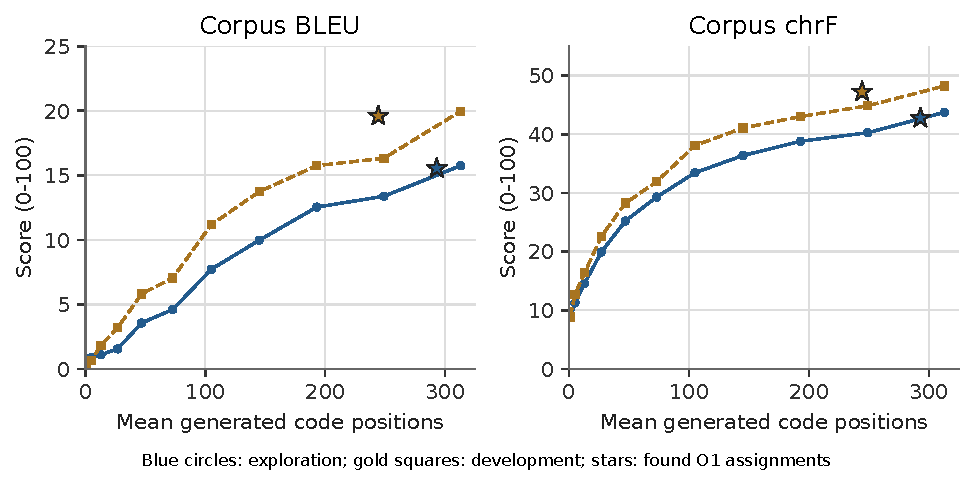
\includegraphics[width=\linewidth]{figures/quality-work.pdf}
\caption{All 11 saved fixed-depth corpus points, with found O1 mixed assignments. Horizontal position is generated-code work, not FLOPs or latency. Stars are feasible points found, not a certified frontier; corpus quality intervals are reported separately.}
\label{fig:frontier}
\end{figure}

On development, O1 selects early exits on 18/64 inputs, mean level 9.28125 and mean 244.34375 codes, versus 11 and 313. O0/O1/O2 happen to retain identical vectors within each split. The development mixed corpus scores 19.59525 BLEU /47.23513 chrF, compared with full 19.96568 /48.21990. Point losses of 0.37043 /0.98477 satisfy the margins. Numeric F1 is unchanged and negation mismatch rises 0.015625.

\begin{table}[ht]
\centering\small
\begin{tabular}{lrr}
\toprule
Development O1 quantity & Point difference/reduction & Conditional 95\% interval\\
\midrule
Corpus BLEU difference &-0.37043&[-1.35104,+0.57282]\\
Corpus chrF difference &-0.98477&[-2.13670,-0.20140]\\
Surrogate cost reduction &9.016\%&[2.799\%,15.778\%]\\
\bottomrule
\end{tabular}
\caption{Conditional estimates versus full and selected fixed depth 11. The one-sided 95\% quality lower bounds are -1.16378 BLEU and -1.90548 chrF, outside the allowed -0.5/-1.0. No actual latency is measured for these assignments.}
\label{tab:primary}
\end{table}

\begin{figure}[ht]
\centering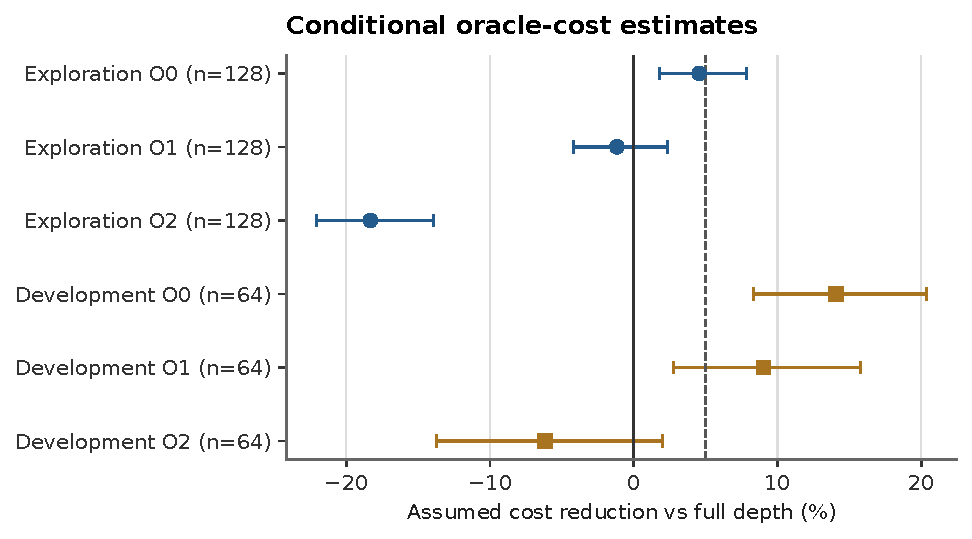
\includegraphics[width=\linewidth]{figures/conditional-cost.pdf}
\caption{Fixed-assignment surrogate reductions and conditional paired 95\% intervals. Positive means lower assumed cost. O1 is primary; O0/O2 cannot rescue it. The dashed 5\% reference is a target, not evidence of actual wall-time reduction.}
\label{fig:cost}
\end{figure}

The O1 point estimates meet the surrogate savings threshold but fail conditional quality noninferiority. Development O2 instead estimates 6.19\% overhead. Under the primary $f/\tau$ assumptions, at least 5\% savings requires $h\lesssim0.00896$; actual $h$ is not identified. Historical development guarded stability takes 135.64551 ms versus 132.56760 ms full, 2.32\% overhead, on its two-observation full-depth path. O1 predicts only 0.7\% overhead for that schedule; this does not calibrate arbitrary depths or separate fixed costs.

Practical headroom is consequently \emph{inconclusive}. The search is positive about finite point-feasible mixed output availability, not about a deployed quality--latency advantage. Differences between exploration and development are also confounded by different sample sizes under the same candidate cap: the smaller split permits more coordinate-descent progress.

\subsection{Saved failure diagnosis}
A separately frozen single-pass diagnosis finds exact visible-text agreement with the same input's final translation before level 11 on 17/128 exploration and 13/64 development inputs. Exact agreement of all 64 raw IDs occurs on only 2/128 and 1/64. Rendering and EOS filtering can conceal token differences. These retrospective matches establish neither reference correctness nor a recognizer available online; we construct no additional exit assignment from them.

\begin{figure}[ht]
\centering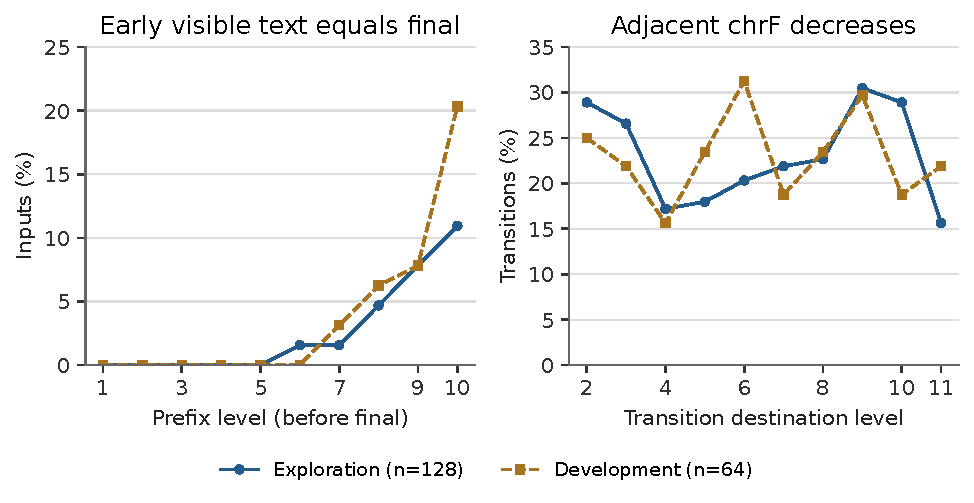
\includegraphics[width=\linewidth]{figures/saved-diagnostics.pdf}
\caption{Saved prefix diagnosis by split: visible equality with each input's own final output, and adjacent sentence-chrF decreases. Final-output matching is retrospective; decreasing reference similarity is not proven semantic harm. These curves are descriptive, without confidence bands.}
\label{fig:diagnosis}
\end{figure}

There are 295/1,280 exploration and 147/640 development adjacent sentence-chrF decreases, despite generally improving corpus scores. Macro reference-word recall is a lexical emergence diagnostic, not a replacement for corpus quality. Of 31/13 number-bearing references, 9/6 have a digit cue missing from every prefix including final. Of 17/9 negation-bearing references, 3/0 lack the required literal cue at every level. Paraphrases, formatting and source/reference differences can create false flags; these are not truth labels.

\section{Interpretation and limitations}
The selected WMT policies have structurally full-depth schedules while some early visible final translations exist. Thus total absence of early translations cannot explain their failure. This supports an availability-versus-recognition distinction without showing that a causal controller can exploit enough of that availability economically.

Representation/decoder limitations remain plausible for Sudoku, but target-encoding results do not isolate a mechanism. Generated-code errors, decoder sensitivity and protocol/measurement constraints remain competing explanations for WMT. No target-encoded WMT control or causal decoder intervention is performed. The new study has cost-sensitivity comparisons rather than model-training ablations; the historical code-feature ablation and its negative scope remain in the preserved v2 report. No internal-state finding applies to all activations; the historical learned-validity model used discrete-code statistics.

The narrow search cannot exclude better oracle assignments. Its sample-dependent progress and selection bias limit statistical interpretation. Corpus feasibility, uncertain noninferiority, literal cues and semantic correctness are different quantities. Reused development, unknown checkpoint overlap and missing document clusters limit generalization. Component/work surrogates are not measured latency, CUDA-stream elapsed or throughput. Historical final comparisons and current diagnostic subsets must not be pooled as independent trials.

The continuation-controller branch does not meet its entry gate. Target-encoding and model-intervention branches are deferred because no result identifies one actionable intervention or resolves the current cost/quality constraints. More experiments solely to obtain a positive result are not justified. A separately priced forced-exit timing proposal is retained but unexecuted; suitable independent quality confirmation would still be required.

\section{Reproducibility and work accounting}
The new saved-data cycle used zero real-checkpoint target encodings, generator requests, decoder forwards, fits or final-outcome access. It charged exactly 60,000 complete search assignments and retained all attempts and accepted vectors. Failed setup import and WSL ownership checks occurred before outcome work and are recorded. No inference was retried. The CPU analysis used the existing Python 3.12 /NumPy 2.5.4 /sacreBLEU 2.6.0 environment and no paid services.

A separate calculation implementation validates all ledger moves/digests/costs, direct corpus points, accepted incumbents and conditional intervals. Retained development timing statistics and diagnosis counts reproduce. The full software suite passes 451 tests. These are implementation checks by the same assistant, not independent researcher review, new scientific observations or hardware replication.

The repository preserves original protocols, source snapshots, empirical records and the v2 report. It includes the new protocols, identity allowlists, assignment/search ledgers, cost sensitivities, diagnosis, check receipts and editable manuscript source. Large checkpoint/data files remain excluded; pinned revisions and digests document availability. Project/package redistribution rights are not inferred from upstream licenses.

\paragraph{Assistance and responsibility.}
Substantial AI assistance was used for implementation, analysis, literature synthesis and writing. Human authors must verify claims, citations, authorship, affiliations, rights and venue disclosures before taking responsibility for submission. No human reviewer approval, author identity, endorsement or acceptance is asserted.

\section{Conclusion}
The frozen saved-data audit finds finite point-feasible early WMT outputs and retrospective early final-text matches, while practical adaptive benefit remains unestablished. Quality uncertainty, uncalibrated cost and bounded search prevent stronger claims. The evidence supports a carefully scoped mixed/inconclusive result and conditional closure of unsupported model work.

\appendix
\section{Pinned execution provenance}
\begin{center}\small
\begin{tabular}{@{}ll@{}}
Upstream source & \texttt{c70274273f489abc73832b2b98584a8483b6b203}\\
Checkpoint revision & \texttt{d342ce8aaea58830eef3b8ad473664673e41f692}\\
Dataset revision & \texttt{6580ba41a4b0a976dde876fbe84d25327617b0e6}\\
Text-tokenizer revision & \texttt{c1899de289a04d12100db370d81485cdf75e47ca}\\
\end{tabular}
\end{center}
No Qwen LM weights are used. Historical inference used RTX 5060, WSL2, float32/eval, four CPU threads and task-specific released sampling. No such inference was rerun for this cycle.

S1 allows 128/64 saved inputs, 10,000 assignments per split/point, no restarts and no bootstrap optimization, within eight allocated CPU-analysis hours and 512 MiB new artifacts. S2A allows one pass over 2,112 states /1,920 transitions, zero model work, within two hours /256 MiB. S5 replays calculations and prepares local artifacts within separate frozen caps. Measured execution receipts, including short actual CPU runtimes, remain distinct from these resource ceilings.

\section{Claim audit}
Established finite observations: no early exact Sudoku solutions in the specified audits; point-feasible mixed WMT assignments found; some early visible text matches final; selected policies run full depth; recorded online comparisons have overhead. Conditional estimates: surrogate savings and fixed-assignment bootstrap intervals. Hypotheses: representation/decoder or generated-code bottlenecks and causal recognition signals. Unsupported claims: actual new speedup, universal impossibility, established mechanism, continuation-model efficacy, safety/factuality guarantees or independent human review.

\begin{thebibliography}{10}
\bibitem{ncm} H. Kumbong et al. Next-Concept Modeling: Fast, Parallel Coarse-to-Fine Text Generation. 2026. \href{https://arxiv.org/abs/2610.14162v1}{arXiv:2610.14162v1}.
\bibitem{dat} M. Elbayad, J. Gu, E. Grave and M. Auli. Depth-Adaptive Transformer. 2020. \href{https://arxiv.org/abs/1910.10073v4}{arXiv:1910.10073v4}.
\bibitem{calm} T. Schuster et al. Confident Adaptive Language Modeling. NeurIPS, 2022. \href{https://arxiv.org/abs/2207.07061v2}{arXiv:2207.07061v2}.
\bibitem{ltt} A. N. Angelopoulos et al. Learn then Test: Calibrating Predictive Algorithms to Achieve Risk Control. 2021/2022. \href{https://arxiv.org/abs/2110.01052v5}{arXiv:2110.01052v5}.
\bibitem{act} A. Graves. Adaptive Computation Time for Recurrent Neural Networks. 2016/2017. \href{https://arxiv.org/abs/1603.08983v6}{arXiv:1603.08983v6}.
\bibitem{ponder} A. Banino, J. Balaguer and C. Blundell. PonderNet: Learning to Ponder. 2021. \href{https://arxiv.org/abs/2107.05407v2}{arXiv:2107.05407v2}.
\bibitem{optimal} S. Becker, P. Cheridito and A. Jentzen. Deep Optimal Stopping. 2020 revision. \href{https://arxiv.org/abs/1804.05394v4}{arXiv:1804.05394v4}.
\bibitem{bestn} Y. Kalayci, V. Raman and S. Dughmi. Optimal Stopping vs Best-of-N for Inference Time Optimization. 2025. \href{https://arxiv.org/abs/2510.01394v1}{arXiv:2510.01394v1}.
\bibitem{reporting} J. Dodge et al. Show Your Work: Improved Reporting of Experimental Results. EMNLP-IJCNLP, 2019. \href{https://aclanthology.org/D19-1224/}{ACL Anthology D19-1224}.
\bibitem{koehn} P. Koehn. Statistical Significance Tests for Machine Translation Evaluation. EMNLP, 2004. \href{https://aclanthology.org/W04-3250/}{ACL Anthology W04-3250}.
\end{thebibliography}
\end{document}
